\documentclass[a4paper,11pt]{article}

\usepackage[utf8]{inputenc}
\usepackage[czech]{babel}
\usepackage[left=2cm,top=3cm,text={17cm,24cm}]{geometry}
\usepackage{graphicx}
\usepackage{listings}
\usepackage{multicol}
\usepackage{url}

\title{Konfigurace a analýza VoIP\\
{\bf\large ISA - Laboratorní cvičení č.4}\\
{\bf\large Prokotol ke cvičení}}

\author{Vysoké učení technické v Brně}

\date{\url{https://github.com/nesfit/ISA/tree/master/lab4-voip}}
\setlength\parindent{0pt}
\begin{document}
{\let\newpage\relax\maketitle}
\vspace{-3mm}
Jméno: \hspace{4cm} Login: \hspace{4cm} Skupina (číslo nebo čas):\\
Datum:

\vspace{-2mm}
\subsection*{1.10 Analýza komunikace peer-to-peer}
\begin{multicols}{2}
  \begin{center}
    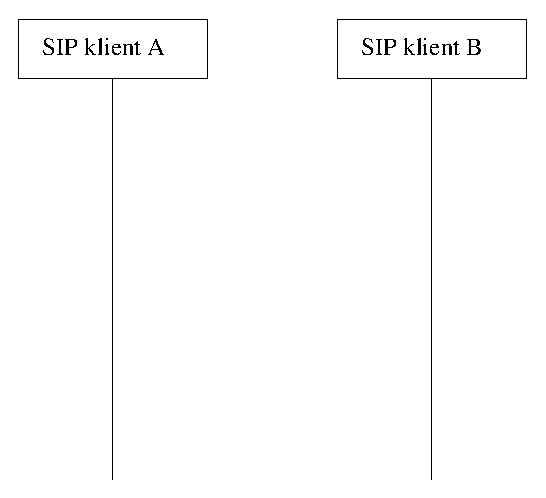
\includegraphics[width=70mm]{img/peer-to-peer.eps}
  \end{center}
  \columnbreak
  \subsection*{Klient A}      
  \begin{enumerate}
    \item Signalizace SIP
    
    \begin{tabular}{lp{2cm}}
      IP adresa a port stanice A: &\\
      IP adresa a port stanice B: &\\
    \end{tabular}               
   
    \item Transport hlasových dat RTP
    
    \begin{tabular}{lp{2cm}}
      IP adresa a port stanice A: &\\
      IP adresa a port stanice B: &\\
      Seznam podporovaných kodeků (pouze čísla):&\\
      &\\
      Použitý kodek (název a číslo): &\\
    \end{tabular}               
  \end{enumerate}      
\end{multicols}

\subsection*{2.1.10 Průběh registrace klienta SIP na ústředně}
\begin{multicols}{2}
  \begin{center}
    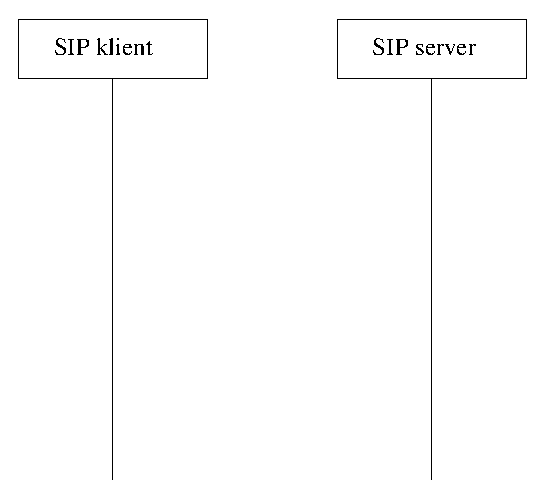
\includegraphics[width=70mm]{img/registrace.eps}
  \end{center}
  \columnbreak
  
  \begin{tabular}{lp{2cm}}
    &\\
    IP adresa a port serveru: &\\
    Název a verze sw serveru: &\\
    &\\
    &\\
    User URI klienta: &\\
    Device URI klienta: &\\
    &\\
    Název a verze sw klienta: &\\
    &\\
    Max. doba přihlášení: &\\
  \end{tabular}               
\end{multicols}
   {\bf 2.1.11} Čím se liší obsah paketu REGISTER při odhlášení od paketu při přihlášení?

\subsection*{2.2.7 Průběh hovoru VoIP přes ústřednu SIP (z pohledu volajícího)}
  \begin{center}    
    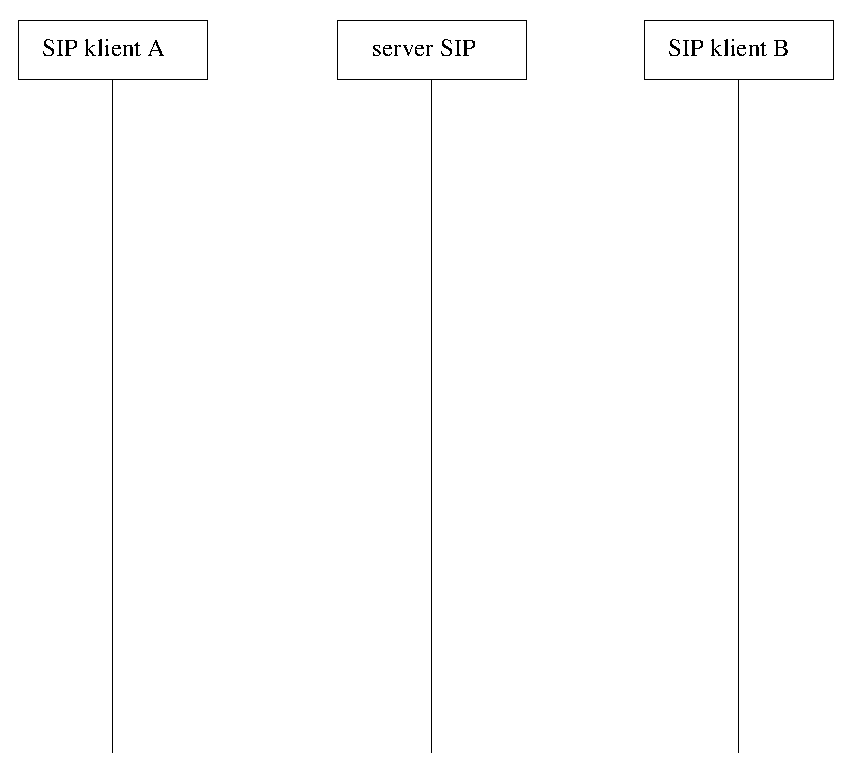
\includegraphics[width=120mm]{img/pres-ustrednu.eps}
  \end{center}
  \vspace{1cm}

  \subsection*{A) Signalizace}
  \begin{tabular}{lp{2cm}}
    IP adresa a port volající stanice A: &\\
    IP adresa a port serveru: &\\
    &\\
    User URI volajícího: &\\
    Device URI volajícího: &\\
    &\\
    User URI volaného: &\\
    Device URI volaného: &\\
  \end{tabular}               

  \subsection*{B) Transport hlasových dat}
  \begin{tabular}{lp{2cm}}
    IP adresa a port RTP volající stanice A: &\\
    &\\
    IP adresa a port RTP volané stanice B: &\\
    &\\
    Vybraný kodek (název a číslo): &\\
    &\\
    Počet přenesených paketů RTP (A $\rightarrow$ B): &\\
    &\\
    Počet přenesených paketů RTP (B $\rightarrow$ A): &\\
\end{tabular}               
\end{document}
